\chapter{图像形成}
\label{chap:rii-image-formation}

\begin{focusbox}{本章复习路线}
从检测任务出发，先定照明、视野与像素分辨率，再把空间点沿“世界坐标 $\to$ 相机坐标 $\to$ 图像坐标 $\to$ 像素坐标”的顺序投影。做尺寸测量时，按标定结果把提取到的像点还原到已知测量面。\textbf{优先练习}相机与镜头选型计算、内外参投影、畸变与标定流程、平面尺寸及圆拟合。
\end{focusbox}

本章对应《第3章：图像形成》讲义。系统组成与选型见 PDF 第10--85页，重点例题见第50--54、75--81页。成像与标定见第103--123页，视觉测量见第124--135页。讲义中的行业案例用于理解任务类型。

\section{机器视觉系统与选型}

典型流程为\textbf{触发采集 $\to$ 照明与成像 $\to$ 图像传输 $\to$ 分析与输出}。触发传感器确定拍摄时机，镜头把场景投到感光靶面，相机完成光电转换与数字化，处理器给出计数、定位、尺寸或缺陷判定。搭建系统时先明确\textbf{想看见哪种差异}，再确定采集参数。

\subsection{照明方式与应用}

\begin{table}[htbp]
\centering\small
\begin{tabularx}{\linewidth}{@{}p{2.5cm} X X@{}}
\toprule
方式 & 成像机制 & 典型任务 \\
\midrule
背光 & 光源位于工件后方，形成高对比度的剪影 & 外轮廓、孔径、液位与遮挡检测 \\
同轴光 & 光经分光元件沿相机轴线照向工件，平整区域的反光进入镜头 & 平整反光表面上的标记或缺陷 \\
暗场光 & 低角度光照射，平面镜面反射绕开镜头，划痕散射入镜 & 低对比度划痕、凹坑及边缘 \\
明场光 & 正面照明，让背景较亮，异常区域产生明暗差异 & 普通表面纹理、字符、灰度对比检测 \\
弥散穹顶 & 从多方向均匀照射，减弱高光与阴影 & 曲面、光泽表面与不规则工件 \\
结构光 & 投射已知光条、点阵或编码图案，利用变形和几何关系测深 & 高度差、轮廓与三维形貌 \\
\bottomrule
\end{tabularx}
\end{table}

光色也会改变灰度对比。以单色相机为例，若表面主要反射红光，红光照明可使红色区域变亮；使用其反射率较低的照明波段可使该区域变暗。实际选择还要看相机的光谱响应和其他区域的反射率。

\subsection{工业相机、视野与曝光}

相机选型先判断单帧的空间覆盖要求。\textbf{面阵}直接输出二维帧，适合固定区域拍照。\textbf{线阵}每次采集一行，依靠物体与相机的相对运动拼成二维图，适合卷材等连续物料。若输送速度为 $v$、沿运动方向所需的物方采样间距为 $q$，则线阵的行频至少为 $v/q$，速度变化时通常用编码器同步。黑白相机便于做单通道灰度测量，依靠颜色区分的任务可用彩色相机与合适的光源。CCD 典型地逐级转移并读出电荷，CMOS 成像单元通常可在芯片内完成放大及分列读出。具体快门方式应看型号。

\dfn{像元、靶面与物方采样间距}{设相机分辨率为 $N_x\times N_y$，每个像元的物理尺寸为 $d_x\times d_y$，则靶面宽高为 $S_x=N_xd_x$、$S_y=N_yd_y$，对角长为 $\sqrt{S_x^2+S_y^2}$。在平行于靶面且可用均匀尺度的测量平面，视野宽高为 $W_x\times W_y$ 时，每像素的物方尺寸为
\[
q_x=\frac{W_x}{N_x},\qquad q_y=\frac{W_y}{N_y}.
\]
若尺寸为 $a$ 的最小特征必须跨越至少 $n$ 个像素，则对应方向 $q\le a/n$，所需像素数 $N\ge\lceil Wn/a\rceil$。位深为 $b$ 的单通道理想量化级数为 $2^b$。}

\textbf{全局曝光}使各行的感光时段一致。\textbf{卷帘曝光}逐行开始或结束，快速运动会使同一帧里的各行记录不同位置，从而产生几何变形。两种快门的单次曝光都可能产生拖影。在物平面内物体以速度 $v$ 匀速横移，若该方向的物方采样间距为 $q$，希望曝光内的拖影不超过 $m$ 个像素，则
\[
t_{\mathrm{exp}}\le \frac{mq}{|v|}.
\]
帧率决定多久取得下一帧，曝光时间决定单帧内积分多久。实际缩短曝光时需同时检查照明、噪声和相机吞吐量。

\begin{figure}[htbp]
\centering
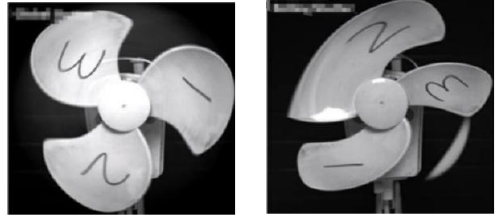
\includegraphics[width=0.46\linewidth]{03-shutters.png}
\caption{转动叶片的全局曝光（左）和卷帘曝光（右）。裁自《第3章：图像形成》PDF 第48页。}
\label{fig:rii-shutters}
\end{figure}

\subsection{镜头、工作距离与景深}

薄透镜模型用物距 $Z$、像距 $s'$、焦距 $f$ 描述合焦条件。沿同一方向设物方视野为 $W$、靶面宽度为 $S$，有
\[
\frac1f=\frac1Z+\frac1{s'},\qquad
|\beta|=\frac{S}{W}=\frac{s'}{Z},\qquad
f=\frac{ZS}{W+S}.
\]
当 $Z\gg f$ 时可令 $s'\approx f$。若题目以工作距离 $\mathrm{WD}$ 近似从镜头主平面量得的 $Z$，则使用讲义中的选型估算 $W\approx \mathrm{WD}\,S/f$。给同一个方向的靶面尺寸 $S$，远距近似下视场角为 $2\arctan[S/(2f)]$。\textbf{固定工作距离和靶面时，焦距越长，视野越小。}

光圈数 $F=f/D$，其中 $D$ 为有效孔径。其余条件相同，缩小光圈（增大 $F$）通常增大景深、减少通光量，成像面照度近似与 $1/F^2$ 成正比。景深是满足清晰度要求的物距范围。尺寸测量若有小幅工件高度变化，可选\textbf{物方远心镜头}使倍率在有效工作范围内对深度变化较不敏感。选镜头还应核对像圈覆盖、接口、畸变和分辨能力。

\Needspace{5\baselineskip}
\ex{从字符笔画估算分辨率、焦距与曝光}{
检测区为 $110\,\mathrm{mm}\times27\,\mathrm{mm}$，需留位置余量，设计视野为 $160\,\mathrm{mm}\times120\,\mathrm{mm}$。最窄笔画宽 $0.5\,\mathrm{mm}$，要求跨过至少 10 像素。靶面宽 $6.4\,\mathrm{mm}$，工作距离约 $400\,\mathrm{mm}$。若工件沿图像水平方向以 $200\,\mathrm{mm/s}$ 匀速移动，按设计采样间距估算允许 1 像素拖影时的曝光时间。
\begin{enumerate}
\item 采样间距上限为 $q=0.5/10=0.05\,\mathrm{mm/pixel}$。取该间距设计，得 $N_x\ge160/0.05=3200$、$N_y\ge120/0.05=2400$，最低约 $7.68$ 百万像素，宽高各自也要达标。
\item 代入远距估算得 $f\approx400\times6.4/160=16\,\mathrm{mm}$。若按理想薄透镜精算，则 $f=400\times6.4/(160+6.4)\approx15.38\,\mathrm{mm}$。实际选接近规格后要复核视野及合焦范围。
\item $t_{\mathrm{exp}}\le0.05/200=2.5\times10^{-4}\,\mathrm{s}=0.25\,\mathrm{ms}$。采用更密的采样时，同一像素拖影限制对应更短的曝光。
\end{enumerate}
}

\nt{“每个特征跨 10 像素”是本例要求。题目给出像素覆盖或定位精度时应按其条件计算，物方采样间距也不能直接作为最终测量误差。镜头与标定误差、噪声、机械振动及边缘定位方法都会影响测量。}

\section{针孔成像与相机标定}

\subsection{四个坐标系与内外参}

\noindent\keypoint{复习重点：外参先把世界坐标变到相机坐标，然后除以相机深度，最后应用内参得到像素。}

设世界点 $\mathbf P_w=(X_w,Y_w,Z_w)^\mathsf T$，使用列向量且规定外参方向为世界到相机。相机坐标为 $\mathbf P_c=R\mathbf P_w+\mathbf t$，其中 $R^\mathsf TR=I$、$\det R=1$。相机中心在世界系中的坐标为 $\mathbf C_w=-R^\mathsf T\mathbf t$，即令 $\mathbf P_c=\mathbf 0$ 所得的位置。

\begin{figure}[htbp]
\centering
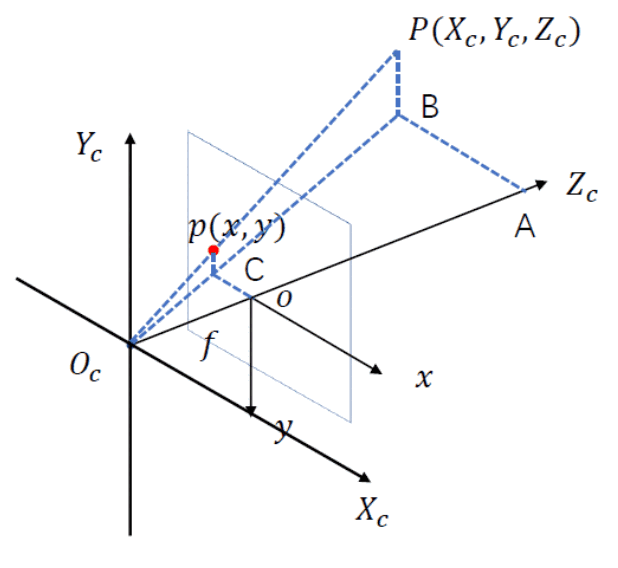
\includegraphics[width=0.51\linewidth]{03-perspective.png}
\caption{空间点与光心的连线在理想像平面上的交点。裁自《第3章：图像形成》PDF 第109页。}
\label{fig:rii-perspective}
\end{figure}

取位于光心前方 $f$ 处的虚像平面，横纵轴与相机系的横纵方向一致。由相似三角形，若 $Z_c>0$，归一化图像坐标为 $(x_n,y_n)=(X_c/Z_c,Y_c/Z_c)$，以长度度量的图像坐标为 $(x,y)=f(x_n,y_n)$。设主点为 $(u_0,v_0)$，像素轴与像面轴方向一致、彼此垂直，则
\begin{align}
u &= \frac{x}{d_x}+u_0=f_x\frac{X_c}{Z_c}+u_0,&
v &= \frac{y}{d_y}+v_0=f_y\frac{Y_c}{Z_c}+v_0,\\
f_x&=\frac{f}{d_x},& f_y&=\frac{f}{d_y}.
\end{align}
$f$ 与 $d_x,d_y$ 用同一长度单位，$f_x,f_y$ 以像素为单位。若题目将某坐标轴定义为相反方向，须在坐标转换中纳入符号。将世界点写成齐次向量 $\widetilde{\mathbf P}_w=(X_w,Y_w,Z_w,1)^\mathsf T$，有
\begin{equation}
 Z_c\begin{bmatrix}u\\v\\1\end{bmatrix}
 =\underbrace{\begin{bmatrix}f_x&0&u_0\\0&f_y&v_0\\0&0&1\end{bmatrix}}_{K\ \text{（内参）}}
 \underbrace{\begin{bmatrix}R&\mathbf t\end{bmatrix}}_{\text{外参}}
 \widetilde{\mathbf P}_w .
 \label{eq:rii-pinhole}
\end{equation}
若考虑像素轴的倾斜，可将 $K_{12}$ 写成非零的斜切项。上述矩阵式描述理想无畸变投影。

\Needspace{5\baselineskip}
\ex{世界点投影到像素}{
已知 $\mathbf P_w=(100,50,2000)^\mathsf T\,\mathrm{mm}$，世界系到相机系的变换为
\[
R=\begin{bmatrix}0&-1&0\\1&0&0\\0&0&1\end{bmatrix},
\qquad \mathbf t=(20,-20,0)^\mathsf T\,\mathrm{mm}.
\]
相机焦距 $f=8\,\mathrm{mm}$，$d_x=4\,\mathrm{\mu m}$、$d_y=5\,\mathrm{\mu m}$，主点 $(640,480)$。求理想像素坐标。

先算 $R\mathbf P_w+\mathbf t=(-30,80,2000)^\mathsf T\,\mathrm{mm}$。由相似三角形得到 $(x,y)=\bigl(8(-30)/2000,8(80)/2000\bigr)=(-0.12,0.32)\,\mathrm{mm}$。换算得 $d_x=0.004\,\mathrm{mm}$、$d_y=0.005\,\mathrm{mm}$，代入得到
\[
u=640-0.12/0.004=610,\qquad v=480+0.32/0.005=544.
\]
光心前方 $Z_c>0$，结果偏向主点左侧和 $v$ 轴正向，符合横纵分量的符号。
}

\subsection{光学畸变与矫正}

径向畸变使离主点较远处的点沿径向偏移，典型表现为\textbf{桶形}或\textbf{枕形}。切向畸变通常来自透镜与感光面的装配偏差。在归一化坐标中，令 $r^2=x_n^2+y_n^2$，一种常用的“理想坐标 $\to$ 畸变坐标”模型为
\begin{align}
L(r)&=1+k_1r^2+k_2r^4+k_3r^6,\\
x_d&=x_nL(r)+2p_1x_ny_n+p_2(r^2+2x_n^2),\\
y_d&=y_nL(r)+p_1(r^2+2y_n^2)+2p_2x_ny_n .
\end{align}
$k_i$ 为径向参数，$p_i$ 为切向参数。随后再以 $K$ 转到像素单位。在仅含 $k_1$ 的该正向模型中，$k_1<0$ 使外侧点向主点收缩，表现为桶形畸变。$k_1>0$ 使外侧点远离主点，表现为枕形畸变。若换成逆模型，应重新根据映射方向判断。矫正单个观测点时需要求正向模型的逆。对整幅图像矫正时，可把输出图上每个理想像素映射到原图，再通过插值采样。

\begin{figure}[htbp]
\centering
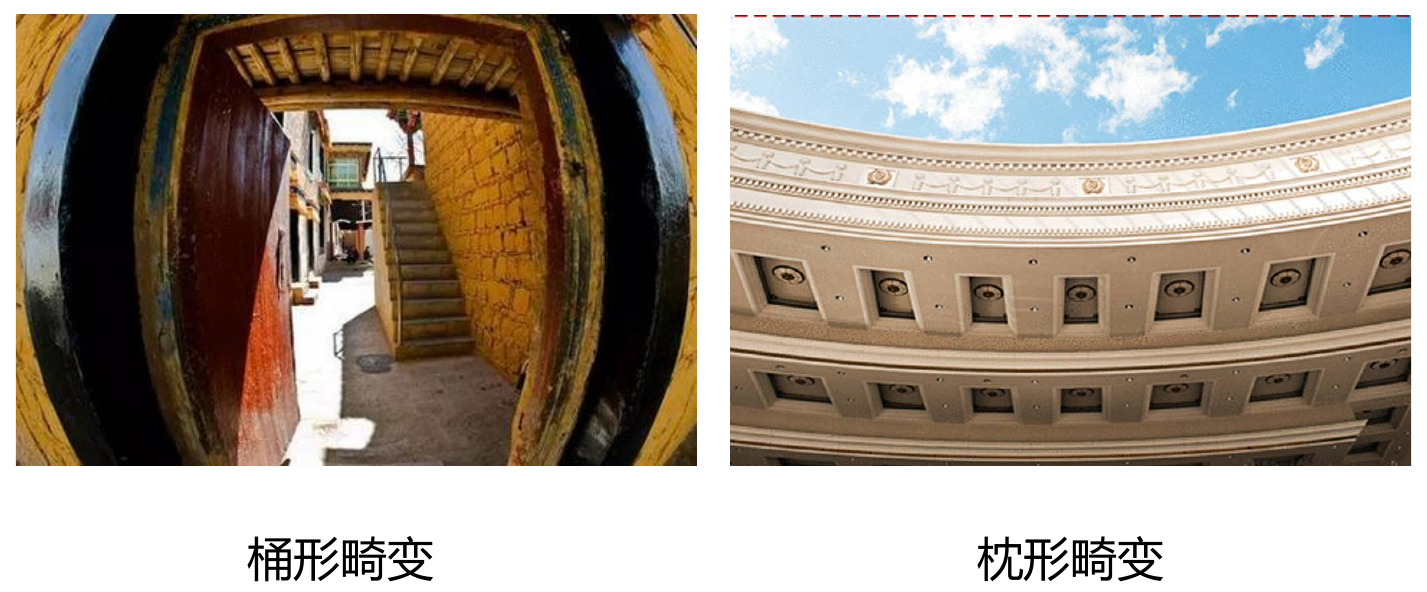
\includegraphics[width=0.88\linewidth]{03-distortion.png}
\caption{桶形畸变与枕形畸变的图像表现。裁自《第3章：图像形成》PDF 第69页。}
\label{fig:rii-distortion}
\end{figure}

\subsection{线性标定、非线性优化与张正友标定法}

\dfn{标定与重投影误差}{相机标定利用一组已知空间坐标及对应像素点，估计内参、外参和畸变参数。将标定点用待估参数投影回像素平面，预测像点与实测像点的像素距离称为重投影误差。其平方和可用作非线性精化的目标函数。}

\begin{enumerate}
\item \textbf{线性标定（DLT）。}令投影矩阵 $M$ 的三行分别为 $\mathbf m_1^\mathsf T,\mathbf m_2^\mathsf T,\mathbf m_3^\mathsf T$，消去齐次比例后，每对匹配点提供两式
\[
(\mathbf m_1-u\mathbf m_3)^\mathsf T\widetilde{\mathbf P}_w=0,\qquad
(\mathbf m_2-v\mathbf m_3)^\mathsf T\widetilde{\mathbf P}_w=0.
\]
$M$ 有 12 个元素，整体比例自由，求一般投影矩阵至少需要 6 对提供足够独立约束的匹配点。点全在同一平面会退化为平面映射问题。
\item \textbf{非线性精化。}可从线性解出发，加入畸变并约束 $R$ 是旋转矩阵，用迭代法最小化 $\sum_i\|(u_i,v_i)-(\widehat u_i,\widehat v_i)\|_2^2$。线性法求初值方便，非线性精化适合描述真实成像。
\item \textbf{张正友标定。}相机设置固定，从多个倾角拍摄已知方格尺寸的平面棋盘，检测角点。取棋盘平面 $Z_w=0$，每幅图满足 $H\sim K[\mathbf r_1\ \mathbf r_2\ \mathbf t]$。利用前两列对应旋转轴的正交性与单位模约束，联合多幅图的单应矩阵求内参，再估各幅外参和畸变，最后精化重投影误差。
\end{enumerate}

\begin{figure}[htbp]
\centering
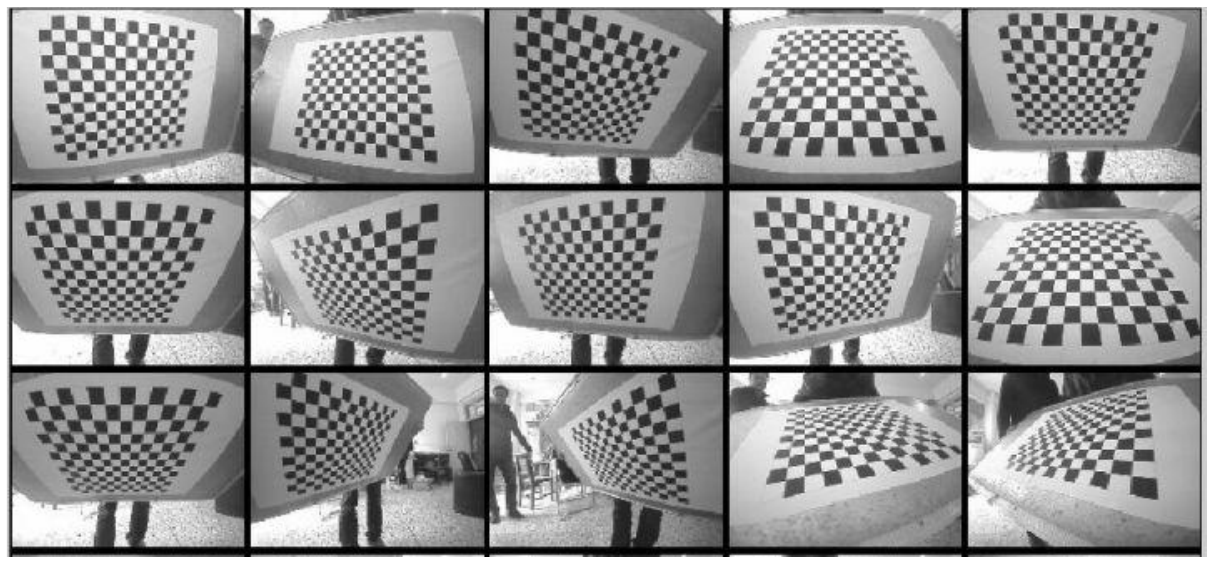
\includegraphics[width=0.75\linewidth]{03-calibration-poses.png}
\caption{相机标定所用的不同倾角与位置的棋盘图像。裁自《第3章：图像形成》PDF 第123页。}
\label{fig:rii-calibration-poses}
\end{figure}

\nt{已知内参时，单个无畸变像素只能确定相机坐标下的一条射线 $\mathbf P_c=Z_cK^{-1}(u,v,1)^\mathsf T$。恢复长度或空间坐标还需要测量平面、深度或多视图等约束。平面标定时应改变棋盘姿态并覆盖视野，留意边缘区域的重投影残差。}

\section{从图像特征到尺寸测量}

平面尺寸测量按\textbf{取感兴趣区域（ROI） $\to$ 去畸变 $\to$ 提取特征 $\to$ 拟合几何模型 $\to$ 转换物理单位}组织。已通过单应矩阵将图像校正到已知平面时，可直接在该平面的物理坐标下算尺寸。若图像已满足均匀比例模型，横纵尺度分别为 $q_x,q_y$ 时，相距 $(\Delta u,\Delta v)$ 的两点距离、由 $N$ 个前景像素组成的区域面积为
\[
\ell=\sqrt{(q_x\Delta u)^2+(q_y\Delta v)^2},\qquad A\approx Nq_xq_y.
\]
倾斜平面或深度变化会改变局部比例。测量齿长等平行边间距时，先将边缘点拟合为共同法向 $(a,b)$ 的两条直线 $ax+by+c_1=0$、$ax+by+c_2=0$，再用 $\lvert c_2-c_1\rvert/\sqrt{a^2+b^2}$ 计算。两条方向向量 $\mathbf v_1,\mathbf v_2$ 的锐夹角可用 $\arccos\bigl(\lvert\mathbf v_1^\mathsf T\mathbf v_2\rvert/(\|\mathbf v_1\|\|\mathbf v_2\|)\bigr)$，若要区分内外角应先确定方向。面积测量可先用连通域标记把各物体分开，再对各域计数。

\textbf{线段端点}可先用 Harris 找角点，再通过拟合边缘精定位。Harris 用窗口平移引起的灰度平方差判断特征，窗口向多个方向移动都产生较大变化时，对应角点。\textbf{Hough 直线检测}用参数式 $\rho=x\cos\theta+y\sin\theta$。单个边缘点在参数空间给出一条曲线；共线的边缘点投票在同一位置聚集。圆的参数为 $(a,b,r)$，每个边缘点对满足 $(x-a)^2+(y-b)^2=r^2$ 的候选投票。已知半径时仅需搜索圆心 $(a,b)$。

\Needspace{5\baselineskip}
\ex{圆轮廓的代数最小二乘拟合}{
在已校正的像素平面中采到四个轮廓点 $(6,2),(0,2),(3,5),(3,-1)$。设圆为
\[
x^2+y^2+A x+B y+C=0.
\]
一般有噪声时，把每点对应的一行 $[x_i\ y_i\ 1]$ 组成矩阵，最小化 $\sum_i[x_i^2+y_i^2+A x_i+B y_i+C]^2$。本例点恰在同一圆上，代入第二点得 $2B+C=-4$；第一点给 $6A+2B+C=-40$，故 $A=-6$；第三点给 $3A+5B+C=-34$，故 $B=-4$、$C=4$；第四点可作校核。配方得到
\[
(x-3)^2+(y-2)^2=9.
\]
圆心为 $(3,2)$，半径为 $3$ 像素。若各方向统一为 $0.20\,\mathrm{mm/pixel}$，物方直径为 $2\times3\times0.20=1.20\,\mathrm{mm}$。代数残差可线性求解，若题目要求最小化实际点到圆弧的距离，应改用几何残差。
}

相机内参和畸变模型为后续视觉控制提供从像素到归一化图像坐标的变换。稳定提取的角点或轮廓可作为图像特征，也可配合目标几何模型估计位姿。

\section{公式速查与自测}

\begin{focusbox}{做题顺序}
\textbf{选型}先确定视野、单像素覆盖、宽高分辨率，再检查靶面与焦距、曝光和照明。\par
\textbf{投影}用 $R\mathbf P_w+\mathbf t$ 计算相机坐标，以 $Z_c$ 归一化，套用畸变模型与 $K$。\par
\textbf{测量}先明确像素与物理平面的对应关系，再找特征、拟合并换算尺寸。
\end{focusbox}

\qs{自测}{
\begin{enumerate}
\item 同时拍摄薄板安装孔和表面划痕，怎样打光？分别说明依据。
\item 已知 $K$、$R$、$\mathbf t$，为什么单个像素无法唯一确定世界点？若目标就在已标定的平面上，怎样求其位置？
\item 靶面为 $8\,\mathrm{mm}\times6\,\mathrm{mm}$，希望在 $\mathrm{WD}=200\,\mathrm{mm}$ 处覆盖约 $100\,\mathrm{mm}\times75\,\mathrm{mm}$，按远距估算应选多大焦距？
\end{enumerate}
}
\noindent\textbf{核对：}（1）背光让孔与板形成轮廓反差。暗场让划痕散射光明显，必要时分时照明拍摄。（2）一个像素给一条反投影射线，将射线与已知平面求交，或求平面单应矩阵的逆变换。（3）从宽或高计算均为 $16\,\mathrm{mm}$。
